% !TeX root = Protokoll.tex
\subsection{Funktionsweise eines Lasers}
\begin{figure}[b!]
	\centering
	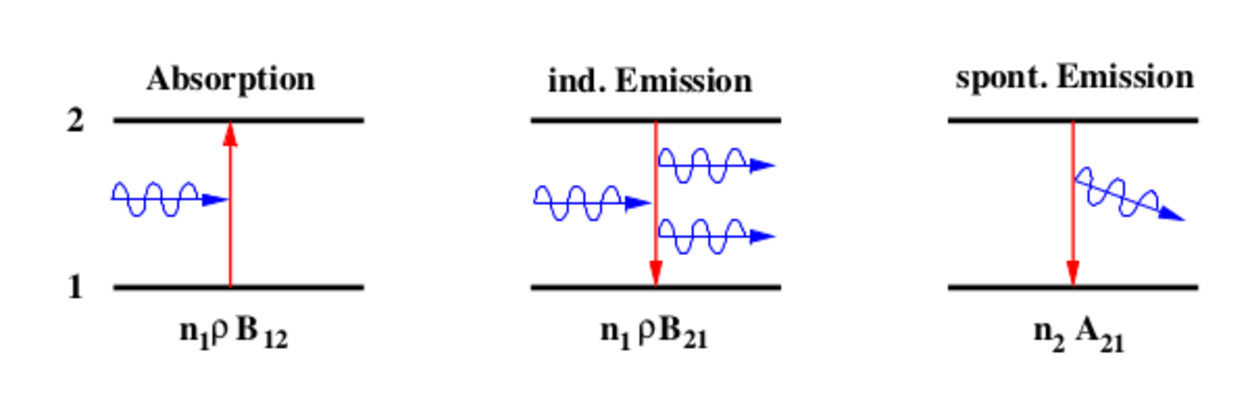
\includegraphics[width = \textwidth]{../Grafiken/Emission.pdf}
	\caption{Hier sind die Emissionen und Absorptionen schematisch dargestellt.\cite{V61}}
\end{figure}
Dieser Abschnitt wurde mithilfe von \cite{V61} erstellt.\\
Grundlegend besteht ein Laser aus drei Komponenten, dem Lasermedium, dem Resonator und einer Pumpquelle.
Die Pumpquelle regt das Lasermedium an, wo durch dies Licht emittiert.
Mithilfe des Resonators wird das Licht öfters durch das Lasermedium geleitet, wodurch mehr Licht emittiert wird das genau die Gleiche Wellenlänge besitzt wie das Licht das es angeregt hat.
Dies hat zur Konsequenz das der Laserstrahl hoher Intensität und  Kohärenz.
Um diesen Prozess genauer zu verstehen, wird das Beispiel eines zwei Niveau Lasers Betrachtet.
Durch ein Photon, das die Energie des Übergangs besitzt, geht das System vom Grundzustand (1) in den angeregten Zustand über.
Die Kohärenz wird dabei durch die Spontane Emission erreicht.
Wenn ein Photon auf das System  trifft, wird ein Photon heraus gelöst, dieses besitzt die selbe Energie, Phase und Ausbreitungsrichtung wie das auslösende Photon.
Dies ist der Effekt der induzierten Emission und der Grund warum Laser so kohärent sind.
Weiter ist es möglich das ein Photon durch spontane Emission emittiert wird, diese Photon besitzt eine Beliebige Phase und Ausbreitungsrichtung.\\
Mithilfe eines Strahlenfeldes $\rho$ lassen sich spontane und induzierte Emission hervorrufen.
Dadurch lässt sich für die Photonenanzahl im System die Gleichungen
\begin{align}
	\dot{N}_A=n_1\rho B_{12}\\
	\dot{N}_{IE}=n_2\rho B_{21}\\
	\dot{N}_{SE}=n_2A_{21}
\end{align}
aufstellen. Hier bezeichnet $n_i$ die Besetzungszahl des Niveaus an, $\dot{N}_A$ ist die Änderung der Photonen durch Absorption, $\dot{N}_{IE}$ die Änderung durch induzierte Emission und $\dot{N}_{SE}$ die Änderung durch spontane Emission.
Weiter sind die Konstanten $A_{21},\ B_{12}$ und $B_{21}$ die Einsteinkoeffizienten und geben die Übergangswahrscheinlichkeiten an.
Es lassen sich daraus nun für den Fall das die Summe der Besetzungszahlen konstant ist die Gleichungen
\begin{align}
	\frac{dn_1}{dt}=&-n_1\rho B_{12}+n_2\rho B_{21}+n_2A_{21}\\
	\frac{dn_2}{dt}=&+n_1\rho B_{12}- n_2\rho B_{21}-n_2A_{21}
\end{align}
aufstellen.
Damit ein Laser dauerhaft Kohärent bleibt, müssen die höheren Niveaus mehr besetzt sein als das Grundniveau, dies wird Besetzungsinversion genannt. 
Das hat zur Folge das spontane Emission seltener auf als die induzierte  Emission.
Um den Zustand der Besetzungsinversion aufrecht zu erhalten, muss dem System dauerhaft Energie hinzugefügt werden.
Dies geschieht zum einem über Die Pumpquelle und zum anderen Durch den Resonator, der das emittierte Licht zurück in das Lasermedium reflektiert, das den Effekt der induzierten Emission hervorruft.
\subsection{Diodenlaser}
\begin{figure}[h!]
	\centering
	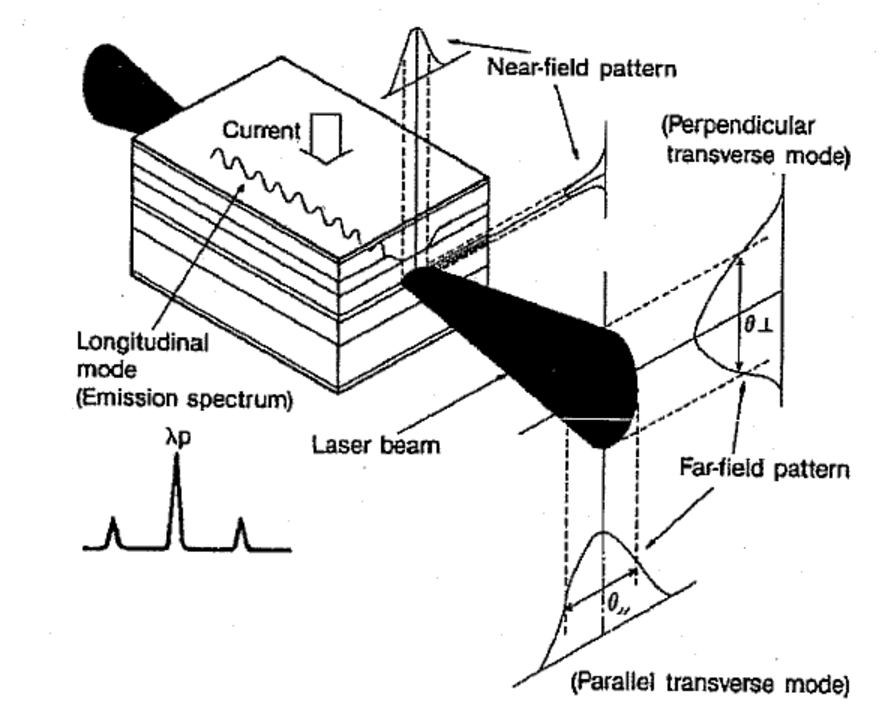
\includegraphics[width = 0.5\textwidth]{../Grafiken/Schematische_Ansicht_Laserdiode.pdf}
	\caption{Skizze des Chips eines Diodenlasers.\cite{V60}}
\end{figure}
Der Diodenlaser kann eine große Bandbreite von Frequenz abdecken $\Delta \nu<\SI{1}{\mega\hertz}$ und auf eine bestimmte Frequenz kalibriert werden. 
In Folgenden sollen die verschiedenen Effekte die dabei eine Rolle spielen behandelt werden.\\
Die Diode fungiert als Pumpquelle, weil sie bei Stromzufuhr Licht emittiert. 
An den Flächen des Chips der Diode befinden sich Spiegel die den Inneren Resonator bilden.
